\section{Vendor independent protocols}
\label{sec:survey_standard}
This section contains a survey on frequently used protocols which offer high bandwidth and reliability. It will be described how the protocols function and how their specifications compare to the requirements mentioned earlier. This section will conclude with a short summary on the discussed protocols and which of them will be the most suitable according to their specifications.

\subsection[The Interlaken Protocol]{The Interlaken Protocol}
	The Interlaken protocol is a narrow, high speed channelized chip-to-chip interface~\cite{InterlakenProtocol}. Interlaken consists of two fundamental structures. These are the data transmission format and the Meta Frame.
	
	The data transmission format relies on the concepts of SPI (System Packet Interface) 4.2 which is a protocol used for data transfer between a link layer and a physical layer~\cite{SPI4.2}. Multiple bursts will contain the data, thus this will not be sent in a single pack. These will be subsets of the original packet data and will be sent sequentially. Before and after each burst, a control word is placed. These words contain important instructions, for example error detection or just an indication of the start or end of a packet. The segmentation of data also allows interleaving of data transmissions from different channels. This can be implemented for low-latency operation.
	
	To transmit the data over a SerDes infrastructure, the Meta Frame is defined. This contains four unique control words to provide lane alignment, clock compensation, scrambler initialization and diagnostic functions. These frames run in-band with the data transmissions, using formatting to distinguish it from the data. In Figure \ref{Fig:Interlaken_Words} the word type structures are depicted~\cite{InterlakenProtocol}.
	
	\begin{figure}[ht]
		\centering
		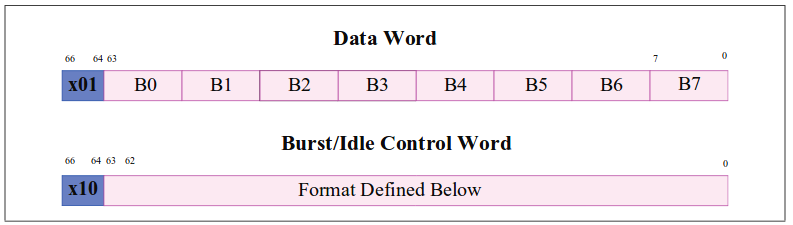
\includegraphics[width=0.7\textwidth]{InterlakenWord.png}	
		\caption{Word formats Interlaken makes use of.}
		\label{Fig:Interlaken_Words}
	\end{figure}
	
	The Interlaken protocol provides a handful of important features:\cite{InterlakenProtocol}
	\begin{itemize}
		\item Support for 256 communications channels, or up to 64K with channel extension 
		\item A simple control word structure to delineate packets, similar in function to SPI4.2~\cite{SPI4.2}
		\item A continuous Meta Frame of programmable frequency to guarantee lane alignment, 
		synchronize the scrambler, perform clock compensation, and indicate lane health
		\item Protocol independence from the number of SerDes lanes and SerDes rates
		\item Both out-of-band and in-band per-channel flow control options, with a simple Xon/Xoff semantic
		\item 64b/67b data encoding/decoding and scrambling/unscrambling
		\item Performance that scales with the number of lanes \newline
	\end{itemize}
	
	Interlaken also features error correction in the form of a 24-bit CRC.
	Instead of the 64b/66b encoding 64b/67b has been chosen to prevent DC balance or baseline wandering. This adds a little overhead but prevents possible bit-errors and complications in the circuitry the receiver contains.\\
	Forward Error Correction has later been added as an extension and offers Reed-Solomon (544,514) encoding. The protocol definition also mentioned the additional overhead. Line coding itself adds about 4,7\% overhead and the RS FEC extension will add an additional about 2,7\% to this which results in 7,5\% overhead~\cite{InterlakenRS}.\\
	
	Both Xilinx~\cite{XilinxInterlaken} and Altera/IntelFPGA~\cite{AlteraInterlaken} developed IP-Cores based on the Interlaken protocol which are capable of achieving huge speeds, 150 Gbps and 300 Gbps respectively. This applies when channel bonding is used. Both vendors claim that a single lane can provide 12,5 or even around 25 Gbps. These speeds would be sufficient according to the requirements and even offer more speed when needed. According to the documentation these cores have recently been updated so they are still maintained which is a good indication.\\


\subsection{SATA protocol}
	Serial-ATA is a communication protocol that evolved from Parallel-SATA~\cite{SATA_Specifications}. Nowadays the technology is often used to for the connection of hard drives~\cite{SATATech}.
	
	Unfortunately the speed of SATA 2 is limited to 3 Gbps and SATA 3 can reach speeds up to 6 Gbps. The maximum speed of SATA 3 is around 0.6 GB/s, the speed current SATA SSD's also reach their maximum read/write speeds.
	SATA-Express is a newer variant of the SATA standard but didn't change much. It is part of the SATA 3.2 standard and actually is just a connector to combine SATA and PCIe~\cite{SATA_E}. An overview of the SATA Express architecture is depicted in Figure~\ref{Fig:SATA_Express_Architecture}~\cite{SATA_E2}.
	
	Thanks to the PCIe support, SATA Express has the ability to use the newer NVMe driver~\cite{SATA_E2}. Unfortunately this is a whole different protocol and actually has nothing to do with the SATA protocol itself, which doesn't reach the required speed and is unsuited for this application.
	
	\begin{figure}[H]
		\centering
		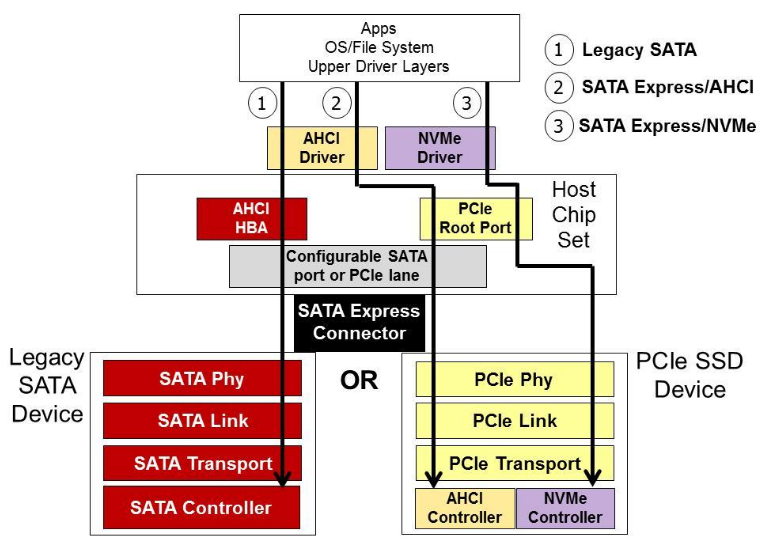
\includegraphics[width=0.6\textwidth]{SATA_NVMe.png}	
		\caption{Overview of the SATA Express architecture.}
		\label{Fig:SATA_Express_Architecture}
	\end{figure}
\newpage


\subsection{CPRI} 
	Common Public Radio Interface is an initiative protocol which was meant to define a publicly available specification~\cite{CPRI_Specification}. This would standardize the protocol interface between the radio equipment control (REC) and radio equipment (RE) in wireless base-stations. It is designed with an optical or copper transmission line in mind. \\
	
	CPRI offers high lane rates up to 24,330 Gbps while using a serial connection. The two most common ways of encoding are used, 8b/10b and 64b/66b are supported. 8b/10b maxes out at 9,8 Gbps and from there on 64b/66b starts to increase the line rate up to te earlier mentioned 24 Gpbs. Speeds of 10,1 and 12,2 Gbps are also possible.\\
	According to the documentation the physical layer is designed in such way that bit errors are very uncommon. This is why error detection is not directly included in the framing or encoding but is more an optional feature. Detection of sync header violation is used to detect link failures in case this occurs.\\
	Unlike CRC which is not mentioned, Forward Error Correction is an optional feature in this protocol.
	
	\begin{figure}[H]
		\centering
		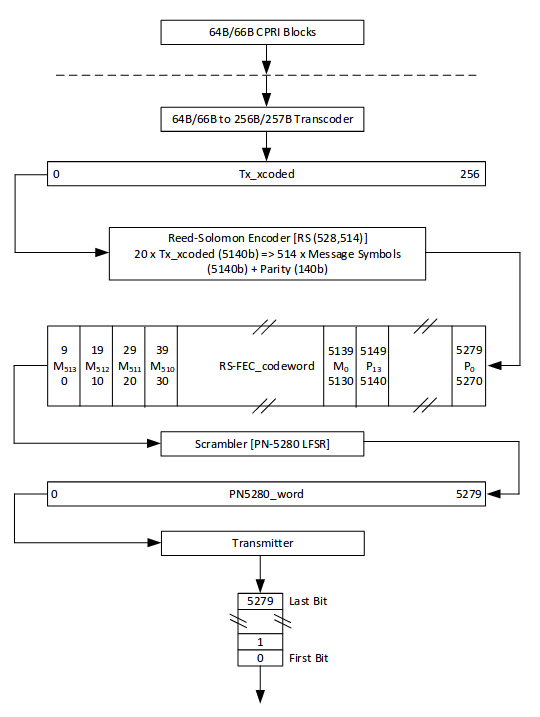
\includegraphics[width=0.58\textwidth]{CPRI_64b.png}	
		\caption{Overview of the CPRI architecture using FEC.}
		\label{Fig:CPRI_Architecture}
	\end{figure}
	
	In Figure \ref{Fig:CPRI_Architecture} the architecture of CPRI uses is visualized~\cite{CPRI_Specification}. It is clearly visible that the data is packed into 66b blocks thanks to the 64b/66b encoder. But these CPRI packets are put into a block of 257b. This is like the earlier explained 256b/257b encoder. These are encoded again by the RS(528,514) FEC, scrambled and transmitted.
	
	There are two different protocols available for the Control and Management (C\&M) information exchange. The slow High level Data Link Control (HDLC) and the faster Ethernet variant. 
	Unfortunately flow control is only available to use for the slow C\&M channel. Selecting HDLC or Ethernet is purely optional. The specifications recommend to support at least one non-zero C\&M channel bit rate on a link~\cite{CPRI_Specification}.
	
	Altera and Xilinx both developed their IP Cores for the CPRI protocol.\\
	So in short CPRI offers the required speed and delivers line rates up to 24,330 Gbps. It doesn't mention CRC but offers the addition of FEC. Flow control is support but only when using HDLC. Channel bonding is not mentioned and the range depends on the cabling.


\subsection{HyperTransport}
	This is a frequently used packet-based, high-bandwidth, scalable, low-latency point-to-point interconnect technology~\cite{HyperTransport_Specifications}. The purpose of this technology was to increase the communication speed between integrated circuits in for example computers, servers and embedded systems.
	Hereby the number of buses is a system can be kept at a minimum, which can reduce the occurrence of possible system bottlenecks. HyperTransport is an open standard which is royalty-free managed. Before implementing HyperTransport a license is required which can be provided by the developers. Figure~\ref{Fig:HyperTransport_Versions}~\cite{HTpic} shows the current versions of HyperTransport and their specifications. 
	
	\begin{figure}[h]
		\centering
		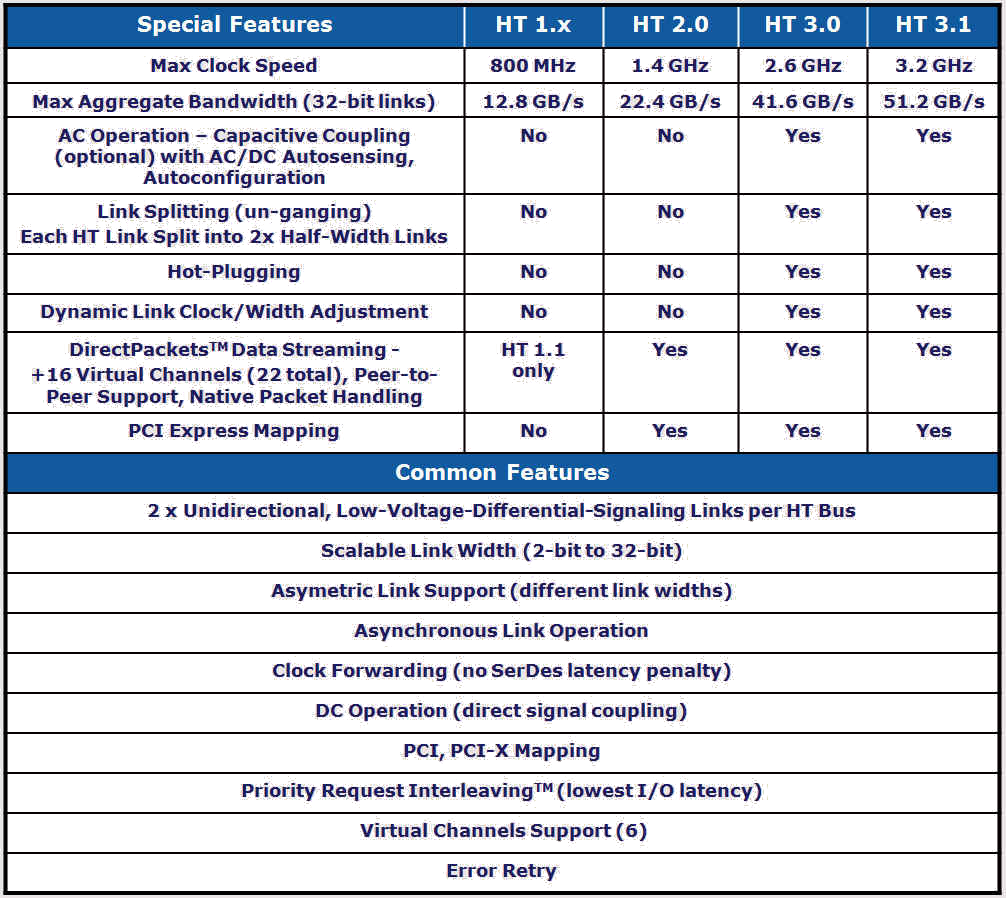
\includegraphics[width=0.7\textwidth]{HyperTransport_2.png}	
		\caption{HyperTransport versions and their specifications.}
		\label{Fig:HyperTransport_Versions}
	\end{figure}
	
	The bandwidth of this protocol is very high but it should be taken in account that this is the case for a 32-bit link. It is possible to make use of the HT point-to-point link using a PCI bus.
	Unfortunately HT has it's own connectors.
	An open-source HyperTransport IP-core has been developed which offers a bandwidth of 1,4GB/s which results in 11,2Gbps~\cite{HTIP}.
	Xilinx used to have it's own IP-Core for HT but unfortunately this has been discontinued. Altera also abandoned it's HT Core and does not recommend use of this IP in new designs. Another paper has been written on a HT3 Physical Layer Interface for FPGA's but unfortunately this reaches proven speeds up to 1600Mbps. The authors claim possible link speeds up to 12,8GB/s but not proven~\cite{HT3IP}.


\subsection{Fibre channel}
	Fibre channel as the name indicates is a communication protocol with optical data transmission kept in mind. The Fibre Channel Industry Association claim it to be a reliable, cost-effective and capable of high speed data transmission~\cite{FC}.
	The recent release variant named 64GFC should reach a throughput of 12,8 GB/s which is sufficient according to the requirements. 128GFC offers a throughput of 25,6 GB/s but is just four parallel 32GFC lanes.\\
	One of the notable things about Fibre Channel is that it makes use of 256b/257b encoding. It packs four control/data words in a single package and adds a header that can be the size of one or five bits. After that a Reed-Solomon Encoder, RS(544,514), is added so it contains FEC. It distributes the symbols and eventually transmits the data using PAM4 technology~\cite{FC64}. \\ 
	
	\begin{figure}[H]
		\centering
		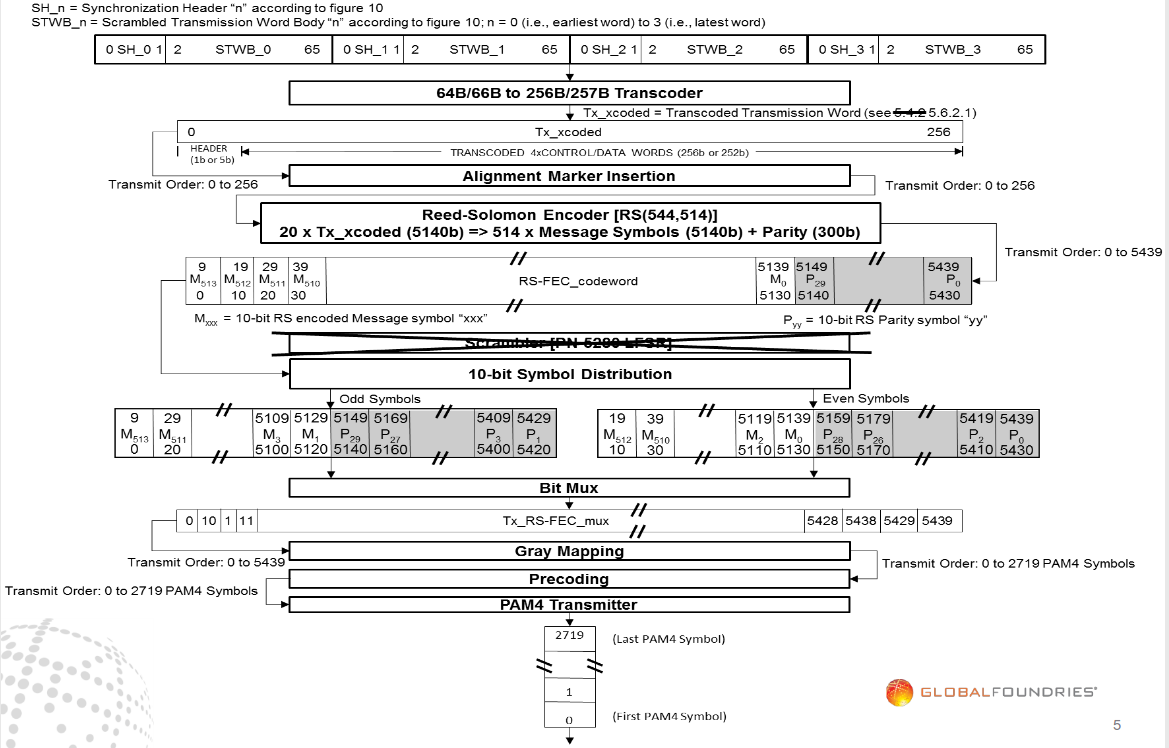
\includegraphics[width=0.6\textwidth]{FC64.png}	
		\caption{Proposed architecture of 64GFC. }
		\label{Fig:FibreChannel_ProposedArchitecture}
	\end{figure}
	
	Figure~\ref{Fig:FibreChannel_ProposedArchitecture}~\cite{FC64} shows a proposed architecture but it's not 100\% certain that this is exactly the same as how it functioned since the official release. However the chance is fairly high it is and slides have been updated through time. Of course this architecture has been well thought through since the source is Global Foundries.
	
	There is not much documentation to be found on the protocol so unfortunately a clear description has not been stumbled upon.
	Xilinx had an IP-Core developed in 2010 for Fibre Channel but unfortunately this IP has been discontinued~\cite{FC_Xilinx}. A newer variant has been released in 2016 but is only available on request and contains an encrypted RTL~\cite{FC_Xilinx32G}.


\subsection{XAUI}
	XAUI is a modern chip interface that came along with the innovations of the 10 Gigabit Ethernet Task Force. The name came into existence by merging AUI from Ethernet Attachment Unit Interface and X (10 in roman numbers) which represents 10 Gigabit. It is designed to extend the XGMII (10 Gigabit Media Independent Interface).
	
	The serial bus used for this interface has a low pin count and is self-clocked. It provides 2,5 times the speed of usual Gigabit Ethernet. The purpose of this protocol is to combine four of these lanes to a single 10 Gbps line~\cite{XAUI_10gea}.
	
	This unfortunately concludes that it is not possible to use a single lane to transfer around 10 Gbps of data. In addition there is still a 8b/10b encoder which can be substituted by a 64b/66b encoder. This could prevent the rather big overhead that comes with 8b/10b encoding. One of the biggest downsides is that the protocol lacks flow control which is an absolute must have~\cite{XAUI_AT}.
	
	Altera/IntelFPGA, Xilinx and Lattice have developed IP cores to implement XAUI in a simple way on your FPGA. Broadcom released HiGig which is used to enhance the XAUI PHY. It makes use of different headers and increases the speed to 6,375 Gbps per lane~\cite{HiGig}.

%\subsection{SPI4.2}
%SPI4.2 offers advantages in channalization, contains programmable burst sizes and per-channel backpressure. Unfortunately the high width of the interface and the source-synchronous features of the protocol reduce the effective reach.


\subsection{Conclusion}
	This section will conclude which of the earlier described protocols is more suitable and whether or not it meets the requirements. Table~\ref{Tab:Survey_Stardard_Overview} provides a quick overview of their specifications. In case a yes is noted, this means support is available but the exact specifications have not been described clear enough. When there is a '-' noted, there is no support or documentation has not been clear enough to provide the required information. 
	All mentioned protocols and links to their documentation can be found in Appendix \ref{Appendix:Protocol_links}.
	
	\taburowcolors[2] 2{tableLineOne .. tableLineTwo}
	\tabulinesep = ^2mm_1mm
	\everyrow{\tabucline[.3mm  white]{}}
	
	\begin{table}[H]
	%\begin{center}
		\begin{tabu} to \textwidth {>{\bfseries}l l l l l}
			\tableHeaderStyle
							& Interlaken 	  & SATA 	& CPRI 			 & Fibre channel \\ 
			Lane rate		& 25,3 Gbps 	  & 6 Gbps 	& 24,33 Gbps 	 & 12,8 Gbps	  		\\ 
			Encoding 		& 64b/67b 		  & 8b/10b 	& 64b/66b		 & 256b/257b 	 	    \\
			Flow control 	& Yes 			  & Yes 	& - 			 & - 					\\
			Range distance 	& Cable dependent & Short	& Cable dependent& Cable dependent		\\
			CRC 			& CRC-24/32		  & CRC-32 	& - 			 & Yes 			   	    \\
			FEC 			& RS(544,514)-Ext & - 	 	& RS(528,514)  	 & RS(544,514) 			\\
			Channel bonding & Upto 400 Gbps   & - 	 	& -				 & - 					\\
		\end{tabu}
		\caption{Overview of the most suited protocols.}
		\label{Tab:Survey_Stardard_Overview}
	%\end{center}
	\end{table}

	SATA is an interesting protocol but the line rate is insufficient. HyperTransport is great for huge bandwidths but implements a parallel bus while serial transmission is required in this case. Fibre channel looks like an interesting alternative. Unfortunately the lack of documentation and not being open will bring a lot of risks with it.
	
	CPRI is another very interesting option offering a high line rate and a good way of encoding. Unfortunately the unclear documentation on CRC and flow control plus the lack of channel bonding cause this option to be a less suited option. Nevertheless a protocol to keep in mind.
	
	The Interlaken Protocol comes out best. While having excellent documentation, the protocol also meets all the requirements. Even the optional/ nice to have specifications. Interlaken is open to use and is even promoted to use by Cortina Systems and Cisco Systems.
	
\newpage
